% source: 论文起草.md L79-L478
\section{模型的建立与求解}\label{sec:model}

\textit{说明：大部分关键数学符号会在正文中随用随引。完整变量清单见附录}

\subsection{第一问：集中式 AIDC 的最大可持续规模}\label{sec:q1}

\subsubsection{可持续规模上限}\label{sec:scale}

我们考虑最大可持续规模，根据题意，是指 \textbf{给定的地区地理条件与资源所能支持单个集成AI数据中心正常运营的最大规模，以技术设备所需电力容量兆瓦度量。}

\begin{noteblock}
\textbf{集中式 AIDC}：本研究沿用题目对 AIDC 的定义，将“集中式 AIDC”界定为主要 IT 设备集中部署于单一场址或地理相邻园区，并由相应的供配电和冷却基础设施支持运行的设施整体。其中，IT 设备包括服务器、GPU 等加速设备、存储及网络设备；供配电损耗、冷却等辅助需求另行核算。
\end{noteblock}

“最大可持续规模”的核心决定因素是什么？在具体抽丝剥茧前，我们先从\textbf{集成AI数据中心}的可持续运行\textbf{状态}开始讨论。一个运营中的AI数据中心会用到以下生产要素：

从中，我们可以先概括出\textbf{能源约束，水资源约束与土地约束}这三项核心约束，它们在给定地理条件下是\textbf{确定且有限}的，而三者共同决定这片土地到底能支撑多大的AI数据中心。

\begin{asum}[固定场址与建成配置]\label{asum:fixed}
模型只考虑某一给定场址的建成状态，认为所有候选设施视为已经建成并处于设计运行状态。对于地理条件，允许出现正常的日夜、季节性波动等，认为不存在长期大范围变更。
\end{asum}

\begin{asum}[正常运营]\label{asum:normal}
模型认为所有设施始终处于正常运营条件下，认为运营期不会出现随机不可控事故。枯水、高温和风光低出力属于正常波动，而极端灾害不在基准结果内，必要时作为敏感性情景另行讨论。
\end{asum}

对给定场址，设 $x$ 为一套确定的建设和运行配置，包括供电方式、冷却方式及用地分配。分别计算这套配置在能源、水和土地约束下可支撑的 IT 额定功率 $P_E(x)$、$P_W(x)$ 和 $P_L(x)$，单位均为 MW IT。三项约束须同时满足，因此该配置的容量为

\begin{equation}\label{eq:q1-capacity}
P(x) = \min\{P_E(x), P_W(x), P_L(x)\}
\end{equation}

比较多个候选配置时，设 $X_y$ 为评估年份 $y$ 已具备投运条件的候选集合。建设工期决定方案最早能在哪一年计入。若该集合非空，当年的最大可持续规模为

\begin{equation}\label{eq:q1-pmax}
P_{\max}(y)=\max_{x\in\mathcal X_y}P(x)
\end{equation}

每当发电预留地或设备配置改变，均按同一配置重新计算三项上限，再比较候选方案。用地分配的计算见附录~\ref{apx:c}。

接下来，我们会详细剖析这三大约束中的具体因素与限制机理。

\subsubsection{能源约束}\label{sec:q1-energy}

对于一个集中式AIDC，需要计算园区的\textbf{可靠供电容量}，即在假设~\ref{asum:normal} 的正常运行条件下，经历所选天气和资源波动时，各时段都能维持的恒定设施负荷，单位为 MW。对给定方案 $x$，电力来自当地电网和园区自建电源。两部分均按园区进线处的净功率计量。

\begin{equation}\label{eq:q1-ptotal}
P_{\text{总}}(x)=P_{\text{电网}}+P_{\text{自发电}}(x).
\end{equation}

其中，$P_{\text{电网}}$ 表示项目接入点可持续稳定交付给园区的电功率。；$P_{\text{自发电}}(x)$ 表示电网承担相应负荷后，自建电源能够持续补充的净功率。

\begin{asum}[配套设施能够输送设计功率]\label{asum:facility}
自建电源配备与其净供电能力相匹配的变电设施，园区内部配电系统不会过载。因此，电网购电与自发电均按园区进线处的净功率计量。
\end{asum}

对于园区\textbf{可靠供电容量}，既供给服务器、存储和网络设备，也维持冷却与配电。按照设施侧与 IT 侧分项计量的口径\cite{q1ref01}，设 $k(x)$ 为设计满载时设施总功率与同一工况 IT 功率的比值。将可靠供电容量除以 $k(x)$，即可得到能源约束下的额定 IT 容量。

\begin{equation}\label{eq:q1-k}
k(x)=\frac{\text{设计满载时的设施总功率}}{\text{同一工况的 IT 功率}},
\qquad
P_E(x)=\frac{P_{\text{电网}}+P_{\text{自发电}}(x)}{k(x)}.
\end{equation}

\begin{noteblock}
对每套方案采用固定的满载设计倍率。若仅有同类设施公布的年度 PUE，可用其近似 $k(x)$，并注明取值的设施类型和统计周期。采用年度 PUE 近似设计满载倍率，意味着假设所研究工况下辅助用电占比接近年度平均水平。若高温等条件显著提高冷却功率，该近似可能高估可承载的 IT 容量；逐时工况扩展见附录 A。
\end{noteblock}

对于自发电容量，可以有多种发电方案，我们考虑比较普遍可行的方案：火力发电，风力发电，光伏发电和水力发电。对每种电源，依次回答两个问题：\textbf{当地可布置多少设备，这些设备又能持续供给多少功率？}

\paragraph{火力发电}\label{sec:thermal}

对燃煤或燃气机组，设 $N_j$ 为场址可布置且能同时正常运行的同型号机组数，$p_j^{\mathrm{net}}$ 为单台机组在当地设计条件下的持续净功率，则

\begin{equation}\label{eq:q1-thermal}
P_j=N_jp_j^{\mathrm{net}}, \qquad j\in\{\text{煤电},\text{燃气}\}.
\end{equation}

单机净功率已扣除电厂自身用电。对采用湿冷的机组，若枯水期的冷却水条件限制出力，则采用该工况下能够维持的净功率\cite{q1ref02}。

\begin{asum}[燃气等燃料条件充足]\label{asum:gas}
对当地法规允许建设的燃气方案，假设外部气源及输送设施能持续满足机组的燃料需求，因此燃气方案所得容量为供气充足条件下的可持续电力承载上界；其环境影响由后续用水、土地及碳排放指标另行评价。
\end{asum}

\paragraph{风力发电}\label{sec:wind}

设 $A_{\text{风}}$ 为分配给风电的合格面积，$\rho_{\text{风}}$ 为单位面积可布置的装机容量。按该密度布置时，风电装机 $X_{\text{风}}$ 为

\begin{equation}\label{eq:q1-wind}
X_{\text{风}}=A_{\text{风}}\rho_{\text{风}}, \qquad P_{\text{风}}=\alpha_{\text{风}}X_{\text{风}}.
\end{equation}

对无储能、独立承担恒定负荷的风电方案，设 $X_{\text{风}} > 0$，$P_{\text{风净},t}$ 为时段 $t$ 的可用净出力，$\mathcal T$ 为所选天气样本覆盖的时段。以逐时净出力估算时，保障比例为

\begin{equation}\label{eq:q1-alpha}
\alpha_{\text{风}}=\frac{\min_{t\in\mathcal T}P_{\text{风净},t}}{X_{\text{风}}}
\end{equation}

该比例由样本期出力最低的时段决定。可用面积与装机密度决定可布置的装机量，当地风况和机组特性决定各时段的出力\cite{q1ref03}。若风电与光伏共用电池，则将两者同一时段的出力相加，按附录~\ref{apx:a} 的功率与电量平衡求组合可维持的恒定负荷。

\paragraph{光伏与储能}\label{sec:pv}

光伏装机同样由合格面积和装机密度确定。设 $A_{\text{光}}$ 与 $\rho_{\text{光}}$ 分别为光伏可用面积与装机密度，则充分布置后的光伏装机为

\begin{equation}\label{eq:q1-pv}
X_{\text{光}}=A_{\text{光}}\rho_{\text{光}}
\end{equation}

由于光伏提供能源存在昼夜波动，要提高全天可维持的恒定负荷，还需将白天的富余电转移到发电不足的时段，因此要考虑储能。电池可以将白天的富余电量转移到出力不足的时段，能够维持的恒定负荷取决于白天可充入的电量，以及电池的充放电功率和可用电量。Goiri 等在 Parasol 实验机房中用 GreenSwitch 协调光伏和电池运行\cite{q1ref04}。本文沿用其功率与电量平衡关系，求给定配置在整个考察期内可持续承担的最大恒定负荷。

\begin{equation}\label{eq:q1-storage}
P_{\text{光储}}=
f_{\text{光储}}\!\left(X_{\text{光}},\,\mathcal W,\,
C_{\max},\,D_{\max},\,E_{\text{可用}},\,\eta_c,\,\eta_d\right).
\end{equation}

其中，$\mathcal W$ 包含考察期内当地日照与气温；$C_{\max}$ 和 $D_{\max}$ 分别为电池最大充、放电功率（MW）；$E_{\text{可用}}$ 为扣除应急预留后可动用的电量（MWh）；$\eta_c$ 和 $\eta_d$ 分别为充、放电效率。关于该 $f_{\text{储}}$ 的具体信息，请参考附录~\ref{apx:a}

\paragraph{水力发电}\label{sec:hydro}

对适宜开发水电的场址，根据可用流量、净落差和转换效率估算可持续供电功率\cite{q1ref06}。设 $Q$ 为预留生态下泄并满足其他用水需求后可持续通过机组的流量（m$^3$/s），$H$ 为同一工况下的净落差（m），$\eta_{\text{水}}$ 为净发电效率，$X_{\text{水}}$ 为机组装机容量（MW）。可计入园区自发电的水电功率取水能条件与机组容量两者中的较小值。

\begin{equation}\label{eq:q1-hydro}
P_{\text{水}}=\min\!\left\{X_{\text{水}},\,0.00981\,\eta_{\text{水}}QH\right\}
\end{equation}

系数 0.00981 包含淡水密度、重力加速度和瓦到兆瓦的换算。若要求枯水期仍能维持额定负荷，式~\eqref{eq:q1-hydro} 应采用枯水期能同时维持的 $Q$ 和 $H$。推导见附录~\ref{apx:b}。

\subsubsection{水资源约束}\label{sec:q1-water}

我们最终需要得出的是水资源约束下的最大IT功率，为此，需先计算实际用于冷却等用途的现场用水（不包括自发电用水），再通过WUE进行转化。经过单位换算，得出以下模型：

\begin{equation}\label{eq:q1-pw}
P_{\text{W}}= \frac{Q_{\text{现场}}}{24\cdot\mathrm{WUE}}\quad(\text{MW})
\end{equation}

其中，$Q_{\text{现场}}$ 为数据中心正常运营所需的现场耗水流量，包括冷却及辅助设施耗水，不含供电过程的间接耗水。其由数据中心可取用水量上限减去发电耗水求得。$Q_{\text{现场}}$及下文提及其他流量均以m$^3$/day为单位。$WUE$ （水资源使用效率，Water Usage Effectiveness）是同期现场取水量与 IT 用电量之比，其在高温等情况中需要特殊取值，具体见附录D。\cite{q1bref04}

为数据中心提供服务的供排水设施的用电，理论上也应包含在数据中心耗水中，但由于其不及总耗水 0.1\%，将其忽略不计。\cite{q1bref09}

\begin{asum}[取输水条件理想]\label{asum:water-ideal}
当可供流量仅来自河流余量或模型控制点时，暂时假设可设置取水口，取水、处理和输水设施有足够能力，且沿途没有输水损失。
\end{asum}

\begin{equation}\label{eq:q1-qfield}
Q_{\text{现场}}=Q_{\text{DC,max}}-Q_{\text{发电耗水}}
\end{equation}

估算数据中心最多可取用的水流量，需同时考虑水压力与政策两个限制。其中，水压力的物理意义为取水需求占水资源的比例，水压力值越高，数据中心给当地带来的资源竞争越大。\cite{q1bref01}因此耗水后的水压力应当被限制在一个合理范围内。

\begin{equation}\label{eq:q1-qdc}
Q_{\text{DC,max}}= \min\left\{\;Q_{\text{DC,压力上限}},\;Q_{\text{DC,政策上限}}\right\}
\end{equation}

式中，$Q_{\text{DC,max}}$ 是的数据中心最大流量；$Q_{\text{发电耗水}}$ 是自发电水耗流量；$Q_{\text{DC,压力上限}}$ 是设置本地水压力阈值后允许的新增流量；$Q_{\text{DC,政策上限}}$ 是项目适用的取水许可或合同上限。

\paragraph{水压力限制}\label{sec:water-pressure}

水压力在运算中的定义为“耗水量与可用可再生水资源之比”。\cite{q1bref01}对选定河段，在 $Q_{\text{河流}} > Q_{\text{生态}}$ 且各项属于同一时段时，定义本地耗水压力并设置阈值：

\begin{asum}[以河流为主要水源]\label{asum:river}
为简化分析，仅考虑从河流中取水，暂不考虑地下水、跨流域调水及水库调蓄的补充作用。
\end{asum}

\begin{equation}\label{eq:q1-pressure}
S_{\text{水}}=\frac{Q_{\text{其他耗水}}+Q_{\text{DC,max}}}{Q_{\text{河流}}-Q_{\text{生态}}}\leq S_{\text{水}\max}
\end{equation}

式中，$S_{\text{水}}$ 是加入数据中心用水的河段耗水压力；$Q_{\text{其他耗水}}$ 是同一水源及同一时段内，生活、工业、农业等已有用户的净耗水量；$Q_{\text{河流}}$ 是取水河段在扣除所计其他取耗水之前的同一时段基准流量；$Q_{\text{生态}}$是出于环境保护考虑的生态保留水量；$S_{\text{水}\max}$ 是本研究设定的允许压力阈值。

将上式对 $Q_{\text{DC}}$ 求解，可得压力所允许的新增取水上限：

\begin{equation}\label{eq:q1-qdcpress}
Q_{\text{DC,压力上限}}
= \max\left\{0,\; S_{\text{水}\max}\left(Q_{\text{河流}}-Q_{\text{生态}}\right)-Q_{\text{其他耗水}}\right\}
\end{equation}

水源数据缺失时的补偿方法见附录~\ref{apx:e}。

\paragraph{水源可支持的新增取水量}\label{sec:water-avail}

我们计算了河流剩余的可用水量，用以证明水压力产生的上限不会出现取不到的情况。水源可支持的新增取水量可用河流流量减去生态保留流量、其他耗水流量得到。

\begin{equation}\label{eq:q1-qavail}
Q_{\text{可用}}
= \max\left\{0,\;
Q_{\text{河流}}-Q_{\text{生态}}-Q_{\text{其他耗水}}
\right\}
\end{equation}

式中，$Q_{\text{可用}}$为河流中可额外取用的水量；$Q_{\text{河流}}$ 是取水河段在扣除所计其他取水之前的同一时段基准流量；$Q_{\text{其他耗水}}$ 是同一水源及同一时段内，生活、工业、农业等已有用户的净耗水量。各项均使用相同流量单位。保留 $\max(0, \ldots)$ 是因为新增取水不能为负。\cite{q1bref02,q1bref03,q1bref08}

因为 $S_{\text{水}\max}<1$，所以 $Q_{\text{可用}}>Q_{\text{DC,压力上限}}$ 恒成立。

\paragraph{自发电耗水}\label{sec:water-gen}

在AI数据中心设有自发电厂时，园区自建电厂的运行用水应被纳入考虑，计入同一场址的水量预算~\cite{q1bref10}。对电源$i$，取与发电技术、冷却方式及水量预算口径一致的运行用水系数 $c_i$（L/kWh）。设 $\bar P_i$ 为该电源当天实际调用的平均净功率（MW），则日用水量为

\begin{equation}\label{eq:q1-qgen}
Q_{\text{发电耗水}}=24\sum_i c_i\bar P_i
\end{equation}

电网优先供电时，按给定 IT 负载超过电网可供部分的缺口确定自发电调用量，并校核该方案的供电上限。式中 1 MW 持续运行 1 小时对应 1,000 kWh，1,000 L 合 1 m$^3$。若水预算按取水量建立，则 $c_i$ 也按取水量取值。采用净耗水预算时，两者均按净耗水取值。

\subsubsection{土地资源约束}\label{sec:q1-land}

土地模型固定为一个\textbf{静态选址模型}：假设数据中心及其配套设施已经建成，问在某片具体地区，土地条件最多允许建设多少 MW 的 \textbf{IT 设备功率}。

\begin{asum}[静态建成状态]\label{asum:static}
我们认为土地条件牵制下，“最大可持续规模”是给定土地条件，即给定物理土地空间的方位与可用性条件下，某片地区最多可承载的 IT 额定功率。这一数值取决于土地性质，在我们讨论的尺度下不随时间改变，默认为静态。
\end{asum}

\paragraph{候选场址选定}\label{sec:land-site}

为建成可运行的AI数据中心，我们首先需要找到有效的，可用于园区内设施建造的物理空间，也就是土地。

\begin{asum}[固定研究边界]\label{asum:boundary}
主结果只计园区本体及明确归属项目的配套电力设施，不考虑远处发电厂，污水处理厂等间接占地。“园区边界内总用地”，包含机房、园区内部变配电、冷却设施、道路、安全间距及预留的必要配套空间。
\end{asum}

先选定较大的候选地理区域，根据法律划地、地形特点及生态保护规则等因素，排除不可建造的土地。对于剩下的可选土地，考虑土地空间上的连续性，以完整连续的土地作为单个候选场址。由此得到每块连续候选场址的面积 $A_{\mathrm{eff},s}$。

\begin{asum}[可持续]\label{asum:sustainable}
通过城市规划确定行政划地，避开（当下与未来规划的）居住区，工业区，自然保育区等；避开有潜在自然灾害区域，如洪泛区；不考虑后续意外情况可能带来的地区风险，如地震，陨石等。

禁建、适宜性和生态避让标准不随计算结果临时更改。
\end{asum}

具体选择规范见附录~\ref{apx:c1}。

\paragraph{功率与需地}\label{sec:land-power}

考虑实际园区给定土地后IT容量的计算，也就是“这片地能塞进几台机子”——现实中，这一关系取决于园区内的具体建筑规划，采用的设备方案，安全规范等等，因素多且复杂，且每个算力中心各不相同。

但是，在给定工程设计方案下，某一特定园区在扩建过程中很可能会保持相近的机柜功率密度、建筑布局、冷却方式及供配电配置。此时机房和配套设施的面积会新增 IT 额定功率\textbf{按稳定比例增加}；园区入口、管理设施等共用部分的面积则大致固定不变。

我们考虑到，现实中确实可能有数据中心在后续扩建中采用新方案，即$a_s$可能变化。但在计算某一用地理论支持容量上限时，固定 $a_s$ 指向全园区采用最高效平均布局。

因此，我们不妨做出假设：

\begin{asum}\label{asum:homogeneous}
园区采用同质扩张，因此每增加 1 MW IT 功率，新增园区用地大致相同，园区需地可用 IT 额定功率的一次函数近似。
\end{asum}

在这一假设下，我们可以估算给定IT容量所需的土地面积大小：

\begin{equation}\label{eq:q1-areq}
A_{\mathrm{req}}(P_{it})=A_{0}+A_{e}+a_sP_{it},\qquad P_{it}>0
\end{equation}

含义是：启动一个园区先占用固定用地与发电区域，随后需地随功率以线性增加。

这里 $a_{\text{s}}$ 的单位是“公顷/MW IT”，是\textbf{边际扩张的用地强度}；$A_0$ 则容纳初始道路、管理区等固定用地。$A_e$表示园区内规划的自建发电站用地，若只使用电网购电或园区外发电站则置$0$

$a_s$由现实园区规划中IT设施总面积除以IT 电力容量，或者以现实园区扩建前后的IT容量与面积增量算出，具体算法见附录C.2。

\paragraph{最大场址}\label{sec:land-max}

因此，对每一块候选场址：

\begin{equation}\label{eq:q1-pland}
P_{\mathrm{land},s}=\max\left\{P>0:A_{\mathrm{req}}(P)\leq A_{\mathrm{eff},s}\text{ 且布局在该地块内可行}\right\}
\end{equation}

在基础线性模型下，若 $A_{\mathrm{eff},s}>A_{0,s}+A_{e,s}$，则说明选地足够支持IT设施的建设，而当需地与该选地面积一致，即所有土地充分开发时，由式~\eqref{eq:q1-areq} 可得该选地最大支撑IT容量：

\begin{equation}\label{eq:q1-pland-linear}
P_{\mathrm{land},s} =\frac{A_{\mathrm{eff},s}-A_{e,s}-A_{0,s}}{a_s}
\end{equation}

若 $A_{\mathrm{eff},s}<A_{0,s}+A_{e,s}$，则意味着土地面积不足，该场址不能按设定方案建设。

最终，在所有的候选场址方案中，理论最大可支持容量为：

\begin{equation}\label{eq:q1-pl}
P_L=\max_{s\in S}P_{\mathrm{land},s}
\end{equation}

\begin{noteblock}
若一个地区有多个候选场址，应逐址按同一配置计算能源、水及土地上限，取三者中的最小值，再比较各可行场址和配置的联合容量。
\end{noteblock}

\subsubsection{结果讨论}\label{sec:q1-results}

第~\ref{sec:q1-energy}--\ref{sec:q1-land}~节分别处理能源、水资源与土地三类约束，并把它们折算成同一量纲——某一场址可持续供给的 IT 功率。本节用三组证据检验它：阿比林园区做同址、同阶段的基准校核；同一园区内四种电源做等资源对比；四个全球场址做迁移检验。%
% 原稿该脚注（md L974 的 [^ai]: ...）只有定义、正文没有标记位，这里补在本节开头，
% 以免这处内容在转换中丢失；若不需要，整条 \footnote{} 删掉即可。
\footnote{本节写作使用 OpenAI Codex 编码代理（2026 年 11 月 22–23 日），工具与版本信息见文献~\cite{apxref29}。具体环节为：梳理团队既有的场址分析报告、结果表与图件；核对各口径与单位换算关系；按竞赛论文的章节结构与表达习惯组织、改写与润色文字；绘制图~\ref{fig:abilene}、图~\ref{fig:sensitivity}、图~\ref{fig:four-sites} 与附录~\ref{apx:f} 中的图件。全部数值结论与文字定稿由团队成员逐项复核，AI 未参与模型设定与结果计算。}

\paragraph{基准校核：阿比林八栋园区的资源上限}\label{sec:abilene}

得克萨斯州阿比林的 Stargate 园区由 Lancium 与 Crusoe 开发、Oracle 承租，毛地约 $1{,}100$ acre。校核对象限定为 \textbf{2026 年拟建成的 8 栋单体建筑}：每栋 4 个 $25$ MW IT 数据厅，另计每栋 $3$ MW IT 其他负载，合计 $8\times(4\times25+3)=824$ MW IT。选它作主校核场址，是因为供电、取水、供地三项边界分别能在并网披露、税收减免协议与州水资源规划中查到，施工范围另有总包披露可核。\cite{apxref01,apxref02,apxref03,apxref04,apxref09,apxref11,apxref12,apxref13}

基准状态下园区全部使用公共电网，现场燃机仅作应急。代入三项边界得：

供电上限 $P_E=1{,}200/1.41=851.06$ MW IT；取水上限 $P_W=633.07/0.50=1{,}266.15$ MW IT（供水取偏宽情景，2030 年市级规划盈余 $4{,}496$ acre-ft/年全年均摊）；土地上限 $P_L=179.61/0.18655=962.75$ MW IT（$a_s$ 由一期前两栋 $38.43$ ha、$206$ MW IT 标定）。三者取小得 $851.06$ \textbf{MW IT}，电力先触顶。

\begin{figure}[H]
\centering
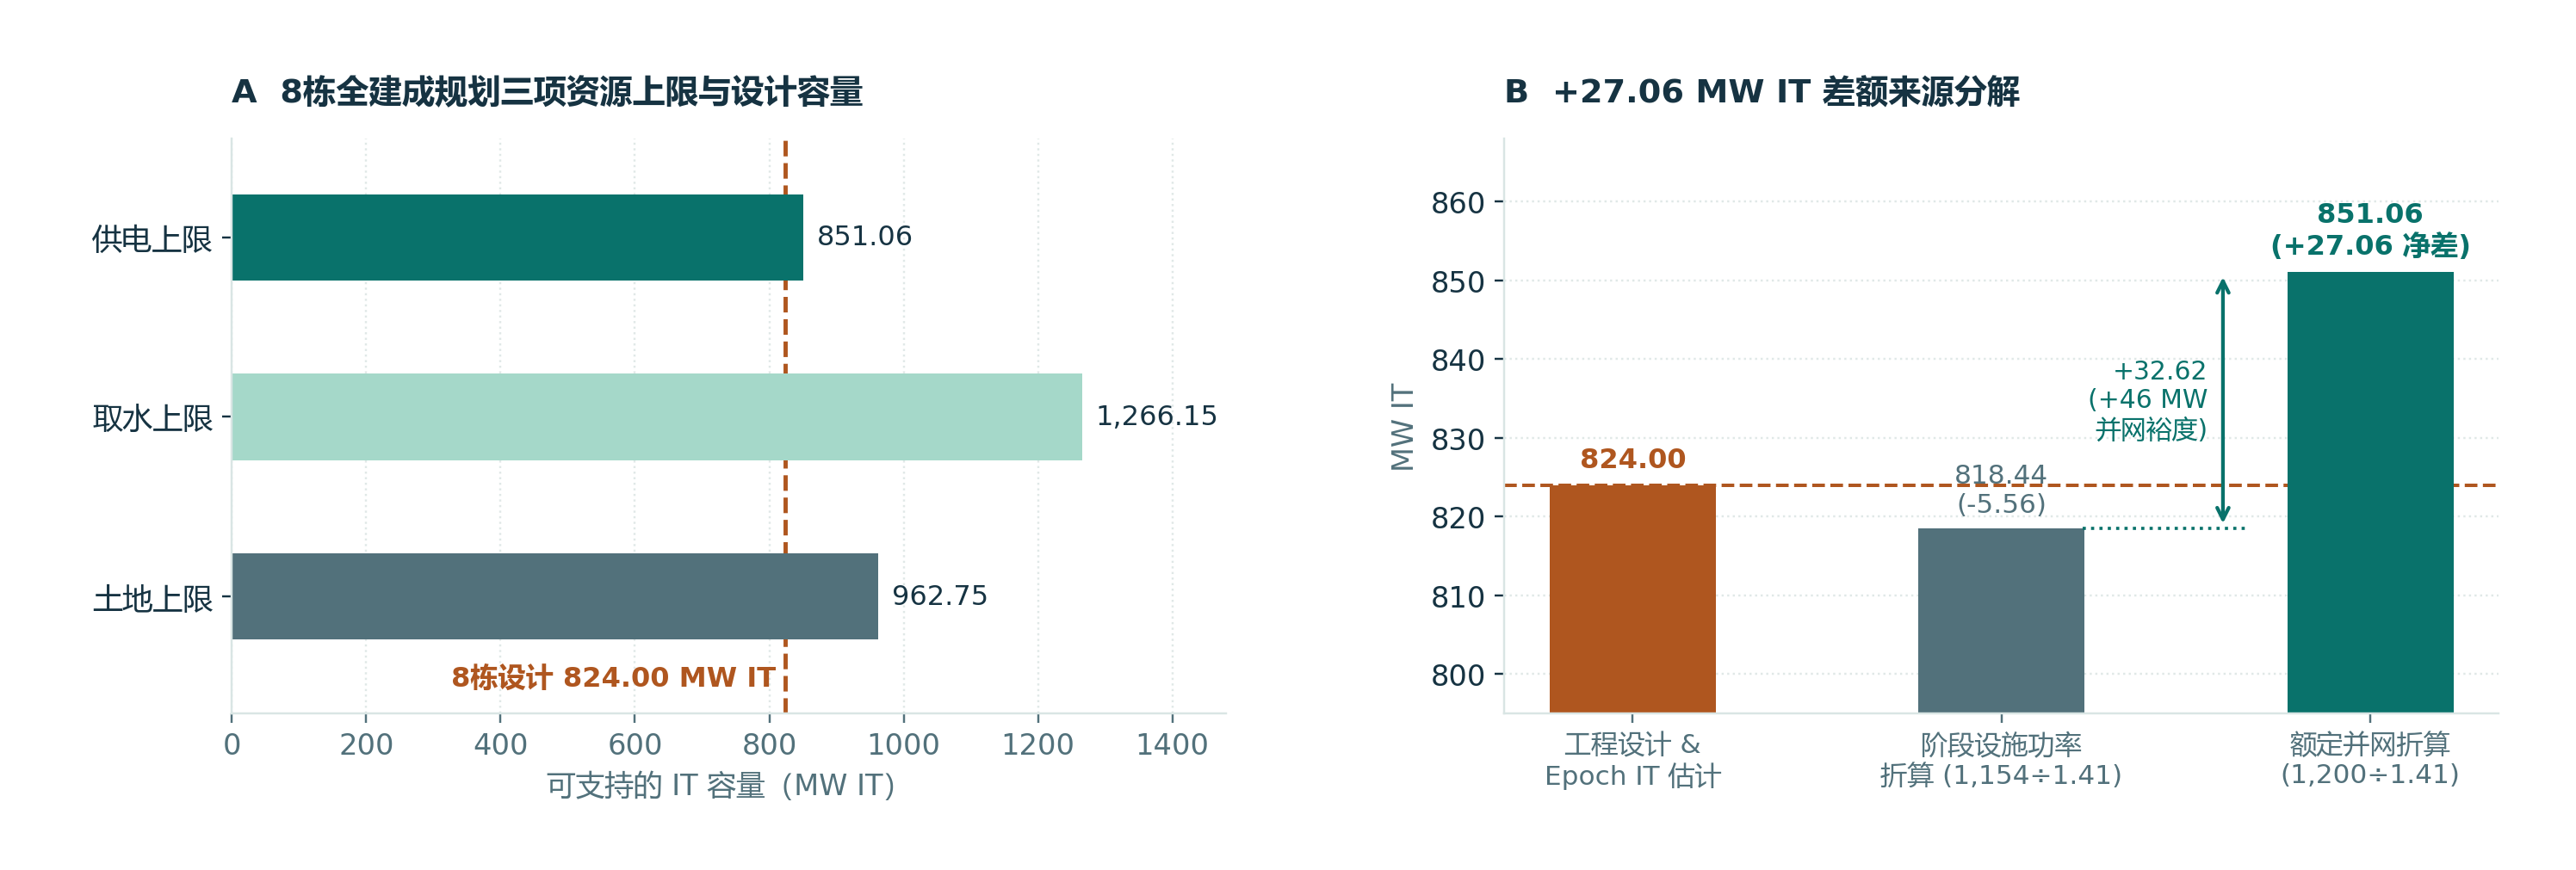
\includegraphics[width=0.76\textwidth]{figures/fig4-1.png}
\caption{阿比林 8 栋建成范围的资源上限与 $27.06$ MW IT 差额分解。左图虚线为 8 栋设备设计 $824$ MW IT；右图三根柱依次为工程设计容量、按阶段设施功率折算的容量、按额定并网折算的容量。}
\label{fig:abilene}
\end{figure}

模型比同阶段设备设计高 $27.06$ MW IT（$+3.28\%$，图~\ref{fig:abilene}）。差额由两段口径差相抵而成：Epoch AI 估计该阶段设施侧功率为 $1{,}154$ MW，低于并网铭牌 $1{,}200$ MW，按 $1.41$ 折算得 $818.44$ MW IT，比设备设计低 $5.56$；铭牌多出的 $46$ MW 裕度则折算为 $+32.62$。两者相抵即 $+27.06$，说明差别来自“额定并网全额交付”与“分阶段实际接入”的口径，而非参数失真。\cite{apxref08}

反过来，$824$ MW IT 满载需 $1{,}161.84$ MW 网电（额定的 $96.82\%$）与 $412.00$ m$^3$/h 到场水；网电只保 $90\%$ 时上限降到 $765.96$，枯季供水收紧到 $400$ m$^3$/h 时瓶颈由电转水、上限降到 $800.00$。本节得到的精度因此是“与同阶段设备设计相差约 $3\%$”，而不是“能预测园区规模”——后者取决于业主分期与并网兑现，不属于资源约束。

把决策边界放宽到允许重排与增建，同一场址的上限落在 $0.85$\textasciitilde$0.98$ \textbf{GW IT}：纯网电 $851.06$；保留既有 8 栋、只在宗地之外的候选地上扩建 $895.60$；2033 年允许重排宗地并投运两台 $100$ MW 干冷燃机则连续分配上限为 $980.75$（按每栋 $103$ MW IT 整栋投运，向下取整为 9 栋、$927.00$）。也就是说，\textbf{对同址同阶段的设备设计偏高 $3.28\%$}；而这个量级与题面所举的 950 MW 档、以及同口径已投运的 New Carlisle（$1{,}037$ MW IT）相当。

\paragraph{同址同水额：煤、气、风、光四种方案}\label{sec:same-site}

题面第一问末要求比较发电方式。我们在同一园区锁定网电 $1{,}200$ MW、可供水 $633.07$ m$^3$/h、$\mathrm{WUE}=0.50$、$k=1.41$，允许在 $179.61$ ha 宗地内重排机房，并开放宗地之外、同属四区块的 $23.36$ ha 候选地用于新建电源；参照题面燃气轮机约七年交付期，对照组设在 2033 年。煤、气按 $100$ MW 整台（占地 $20$、$10$ ha），风光配 4 小时电池（充放功率 $25\%$、效率 $0.90$）。\cite{apxref05,apxref07,apxref14}

\begin{figure}[H]
\centering
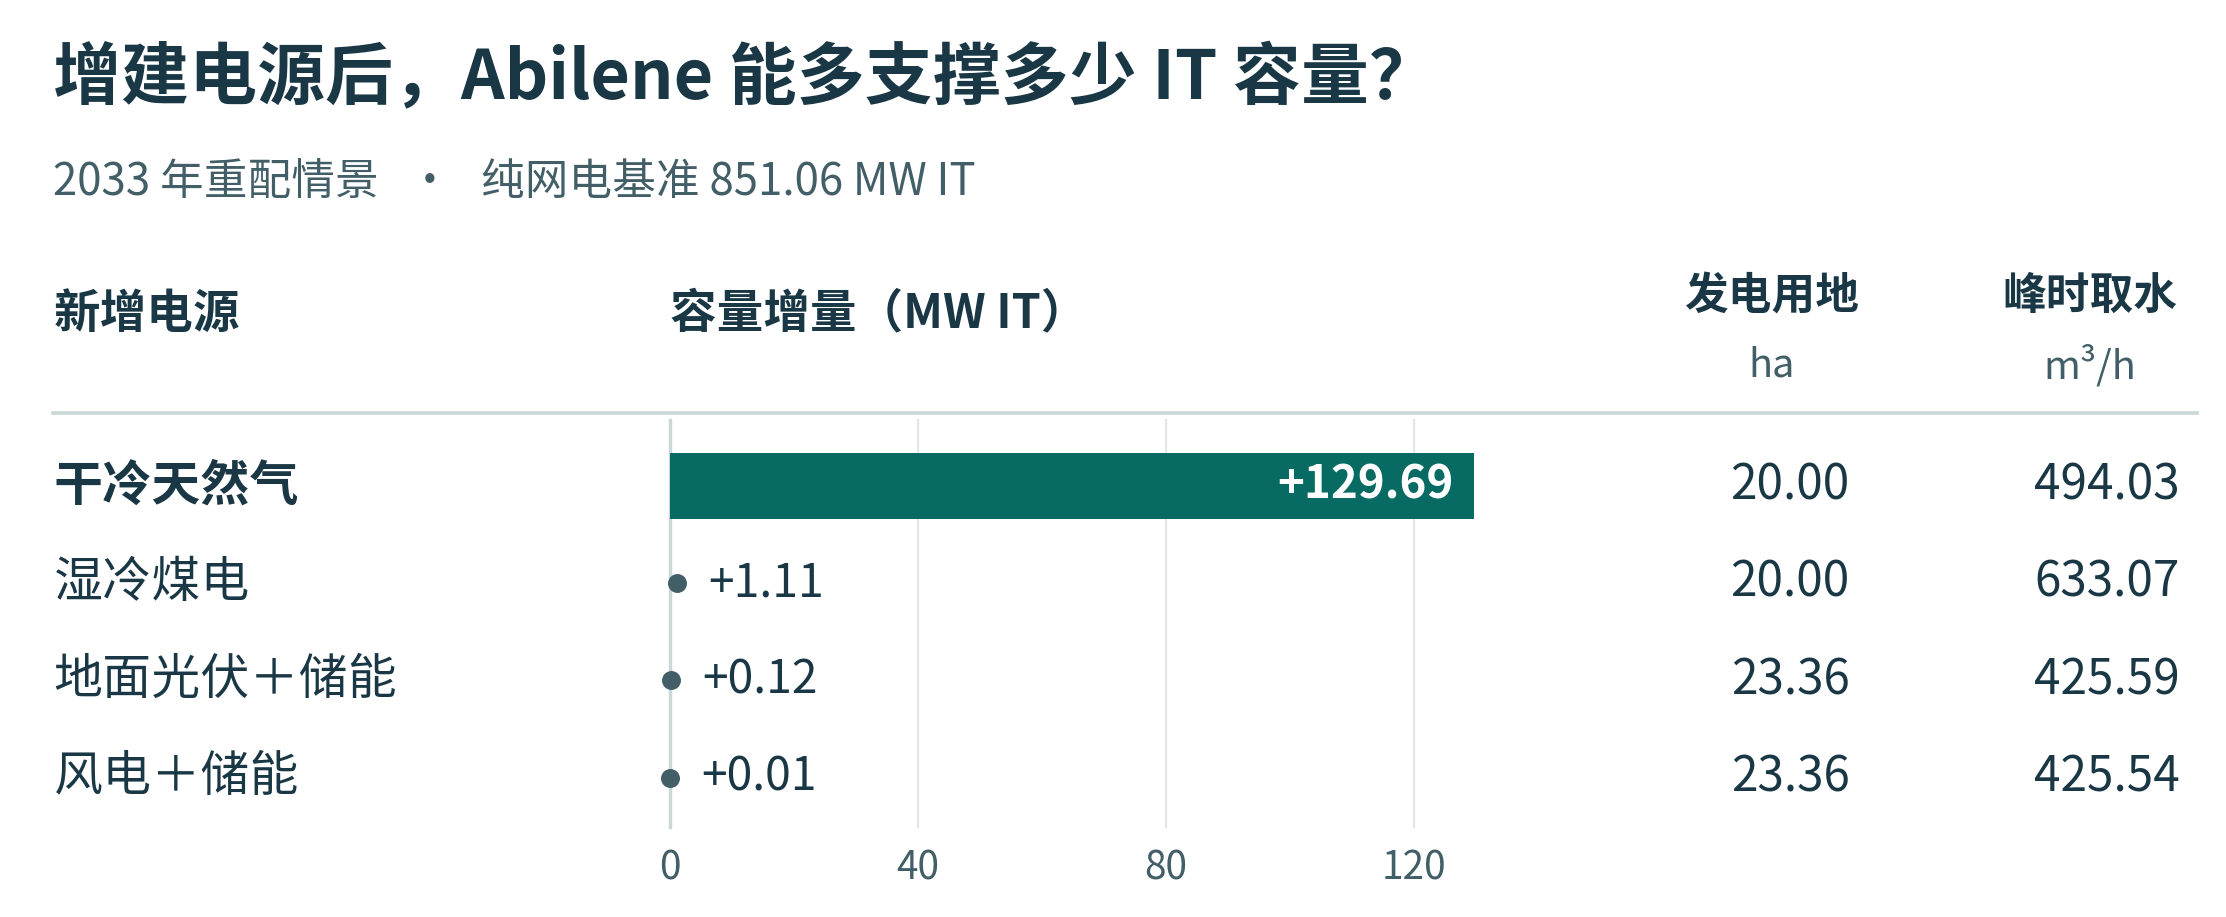
\includegraphics[width=0.76\textwidth]{figures/fig4-2.png}
\caption{同一场址四种增建电源对 IT 容量上限的增量与资源占用。四种电源按增量降序排列；以纯网电基准 $851.06$ MW IT 为零点，右侧两列给出新增电源占用的土地与系统峰时取水。}
\label{fig:sources}
\end{figure}

{\small\setlength{\tabcolsep}{4pt}
\begin{longtable}{@{}p{0.195\textwidth}p{0.085\textwidth}p{0.085\textwidth}p{0.10\textwidth}p{0.115\textwidth}p{0.085\textwidth}p{0.095\textwidth}p{0.06\textwidth}@{}}
\caption{同一电网与供水条件下四种电源的制约机制与容量上限（阿比林 2033 年重配情景）。}
\label{tab:sources}\\
\toprule
供电方案（最优配置） & 发电占地（ha） & 电力上限（MW IT） & 土地上限（MW IT） & 峰时总取水（m$^3$/h） & 最终容量（MW IT） & 较纯网电增量 & 首先触顶 \\
\midrule
\endfirsthead
\toprule
供电方案（最优配置） & 发电占地（ha） & 电力上限（MW IT） & 土地上限（MW IT） & 峰时总取水（m$^3$/h） & 最终容量（MW IT） & 较纯网电增量 & 首先触顶 \\
\midrule
\endhead
\bottomrule
\endlastfoot
纯网电基准 & $0.00$ & $851.06$ & $1{,}087.96$ & $425.53$ & $851.06$ & — & \textbf{电力} \\
湿冷煤电 $1\times100$ MW & $20.00$ & $921.99$ & $980.75$ & $633.07$ & $852.17$ & $+1.11$ & \textbf{水资源} \\
干冷燃气 $2\times100$ MW & $20.00$ & $992.91$ & $980.75$ & $494.03$ & $980.75$ & $+129.69$ & \textbf{土地} \\
风电 $0.78$ MW＋储能 & $23.36$ & $851.07$ & $962.75$ & $425.54$ & $851.07$ & $+0.01$ & 电力 \\
地面光伏 $6.49$ MWac＋储能 & $23.36$ & $851.18$ & $962.75$ & $425.59$ & $851.18$ & $+0.12$ & 电力 \\
\end{longtable}
}

{\footnotesize
\noindent 注：表中“土地上限”按\textbf{允许重排时的总土地盘} $202.97$ ha（运营宗地 $179.61$ ha ＋宗地之外的候选地 $23.36$ ha，见附录~\ref{apx:f1}）计算，与第~\ref{sec:abilene}~节只算运营宗地 $179.61$ ha 的 $962.75$ MW IT 边界不同——候选地一旦被电源占用，被占部分便不能再用作机房用地，故光伏与风电两行按 $202.97-23.36=179.61$ ha 计、土地上限回落到 $962.75$ MW IT；“峰时总取水”为设计日机房与自建电源的合计取水量，不是许可额度。
\par}

四种方案的增量差两个数量级（图~\ref{fig:sources}、表~\ref{tab:sources}：$+1.11$、$+129.69$、$+0.01$、$+0.12$ MW IT），差异由“先消耗哪种资源”决定：

\begin{enumerate}[leftmargin=2em]
\item \textbf{湿冷煤电（$+1.11$）}：机组占 $20$ ha 把土地上限压到 $980.75$，取水系数 $132.5$ L/kWh 又把 $633.07$ m$^3$/h 的水额吃满——机房冷却已用 $426.09$，余额只够机组持续出力约 $1.56$ MW。电和地都没触顶，是水锁死了它。\cite{apxref06}

\item \textbf{干冷燃气（$+129.69$）}：取水强度仅 $0.02$ L/kWh，两台机组占 $20$ ha 后电力上限推到 $992.91$，瓶颈转为土地（$980.75$），实际调用约 $182.86$ MW。前提是气源、环评与宗地重构同时成立；若保留既有 8 栋，只剩 $13.36$ ha 可扩建，即 $895.60$。

\item \textbf{风电与光伏（$+0.01$／$+0.12$）}：$23.36$ ha 只装得下 $0.78$ MW 风机或 $6.49$ MWac 光伏；AIDC 要的是逐时恒定功率而非年均电量，4 小时电池在夜间与低风时段无力平抑。改用未参与求解的 2024 年 $8{,}784$ 小时气象复算，可靠增量也只有 $0.15$ MW IT。\cite{apxref10}
\end{enumerate}

时间维度上四者并不等价：风光 $1$–$2$ 年可建，燃气按题面约七年，故 2030 年前能新增的只有风光（$+0.01$／$+0.12$ MW IT），$+129.69$ 必须等到 2033 年。“时间上能建成”与“电量上够用”在本场址是两个答案。

\paragraph{敏感性与压力测试}\label{sec:sensitivity}

一项结论应当经得起参数与资源的合理变动。我们从单因素敏感性、直接压力情景、跨年气象三个层次检验，结果按影响幅度排列于图~\ref{fig:sensitivity}，逐项网格见附录~\ref{apx:f4}。

\begin{figure}[H]
\centering
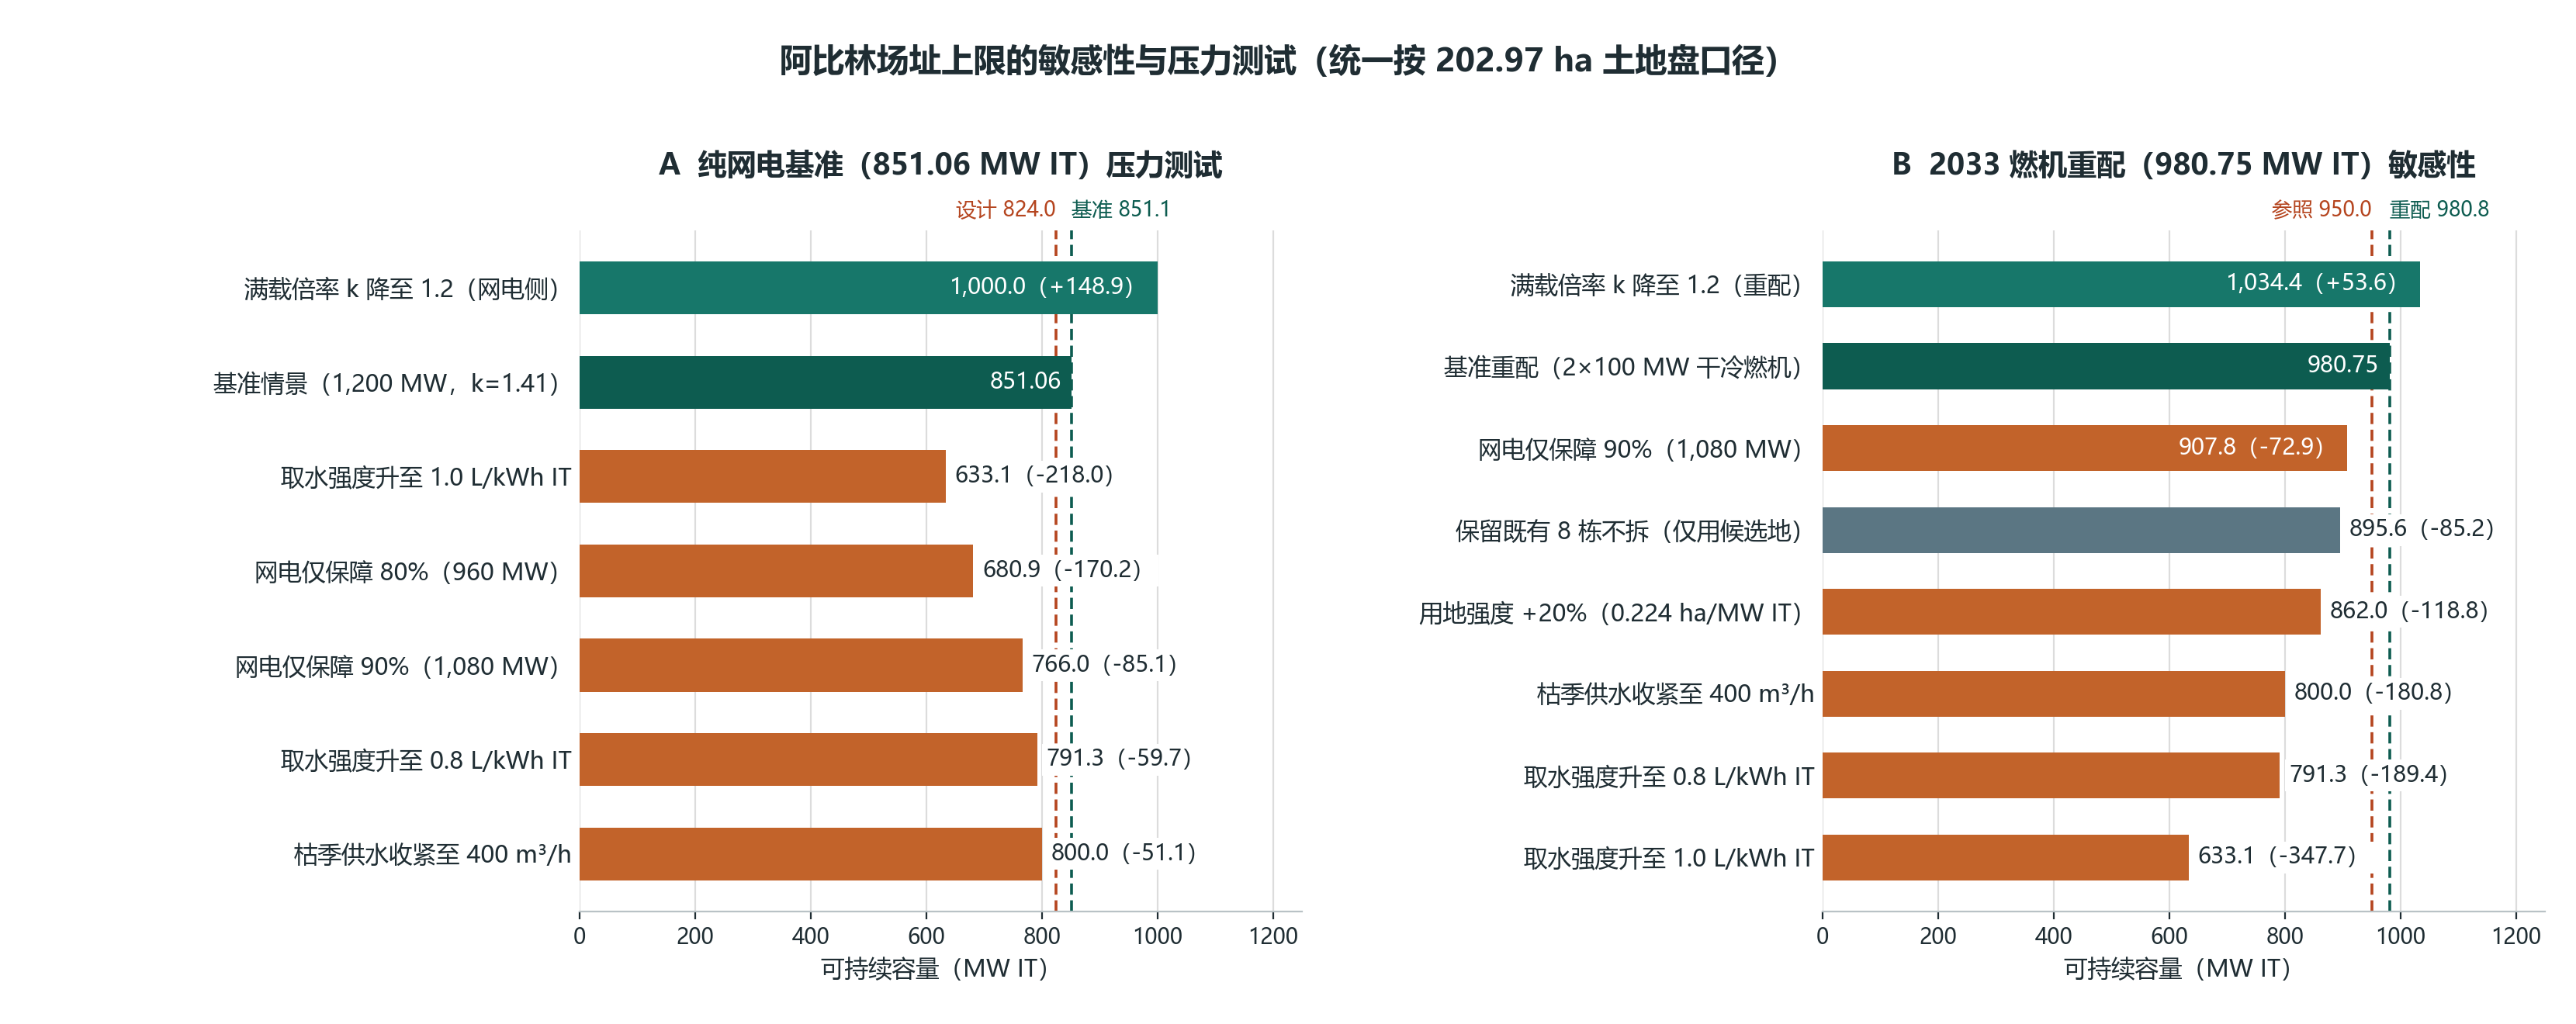
\includegraphics[width=0.76\textwidth]{figures/fig4-3.png}
\caption{阿比林上限的压力测试排序。横轴为可持续容量（MW IT）；左图为“只用网电”的交付边界，右图为“允许重排并投运两台干冷燃机”的边界。两图共用同一横轴量程与同一 $202.97$ ha 土地盘口径。}
\label{fig:sensitivity}
\end{figure}

三点结论。第一，\textbf{水在两条分支上都排第一}：取水强度升至 $1.0$ L/kWh IT，重配分支的全部燃气增益被抹平、回落到 $633.07$，损失 $347.7$ MW IT，比任何电源方案的增量都大。第二，\textbf{参数改善的收益远小于恶化的损失}：$k$ 降到 $1.2$ 只多 $53.6$，一次水质导致的取水强度翻倍却抹掉 $347.7$，扩容应先锁住水再谈电源；且 $k$ 改善带来的是效率余量，不能读作资源变多。第三，\textbf{排序随分支而变}：纯网电分支的主导项是网电交付份额（$80\%$ 时 $-170.2$），重配分支一旦能自建电源，土地变成更紧的约束（用地 $+20\%$ 时 $-118.8$）；枯季供水收紧时瓶颈甚至会由电转水、上限掉到 $800.00$——“哪个约束先触顶”本身随水文年变化。

对 $950$ MW 档：重配分支只要网电保障降到 $90\%$，上限即跌到 $907.82$，低于该档；而 $k$ 改善到 $1.2$、或用地强度下降，都能把它推过 $950$（$1{,}034.36$、$992.92$）。跨年气象检验另给稳健性旁证：设计日可靠增量 $0.1172$ MW IT，2024 年整年复算 $0.1543$，同量级——“小面积风光不足以支撑恒定负荷”不是单日气象的偶然。\cite{apxref10}

\paragraph{迁移检验：四个全球场址}\label{sec:migration}

迁移检验取四处真实 AI 数据中心场址：冰岛凯夫拉维克、新加坡丹戎吉岭、智利基利库拉、澳大利亚悉尼西部，统一按 2030 年条件、2025 年逐时天气运行纯网电与屋顶光储，取较优者作为基准容量。\cite{apxref15}

{\footnotesize
\setlength{\tabcolsep}{3pt}
\begin{longtable}{@{}p{0.14\textwidth}p{0.07\textwidth}p{0.06\textwidth}p{0.29\textwidth}p{0.135\textwidth}p{0.215\textwidth}@{}}
\caption{四个对比场址的 2030 年基准容量、首要瓶颈与公开参照的口径性质。}
\label{tab:four-sites}\\
\toprule
场址与评估边界 & 基准上限（MW IT） & 首要瓶颈 & 同址可核对的公开参照（时点） & 参照的证据性质 & 主要待核缺项 \\
\midrule
\endfirsthead
\toprule
场址与评估边界 & 基准上限（MW IT） & 首要瓶颈 & 同址可核对的公开参照（时点） & 参照的证据性质 & 主要待核缺项 \\
\midrule
\endhead
\bottomrule
\endlastfoot
\textbf{冰岛凯夫拉维克}（Verne 全园） & $100.00$ & 电力 & 首期变电站 $120$ MW（2026 扩建公告）、年 PUE $1.20$（2025 披露）；VDC04 新模块按 $2.4$ ha 布局得 $100$ MW IT（模块密度约 $0.024$ ha/MW IT，高于场地平均 $0.02$）\cite{apxref16,apxref17,apxref18} & 运营披露 ＋ 拟扩建公告 ＋ 布局推算 & 未取得燃料与配气合同；VDC04 达 $120$ MW IT 需扩至 $7{,}200$ m$^2$ 或提柜密至 $120$ kW，并获配 $144$ MW \\
\textbf{新加坡丹戎吉岭} & $110.45$ & \textbf{水资源} & 最高设施需求 $150$ MW（市场研究代理）、预期 PUE $1.19$；供水按等效 DN250 专管 $265.07$ m$^3$/h、当地 $\mathrm{WUE}=2.4$ \cite{apxref19,apxref20,apxref21} & 市场研究代理 ＋ 情景假设 & 无实际配水合同；纯网电口径 $150/1.19=126.05$ MW IT，含屋顶光储为 $126.07$ \\
\textbf{智利基利库拉} & $60.20$ & 电力 & 2025 年电网需求预测 $65$ MW、PUE $1.08$；环评水权 $50$ L/s（$180$ m$^3$/h）；留存单段 $76$ MVA 回路情景 $66.85$ MW IT \cite{apxref22,apxref23,apxref24} & 需求预测 ＋ 环评水权 & 井群实测均值仅 $15$ L/s，对应上限 $20.28$ MW IT；2025 年全址平均取水 $120.2$ m$^3$/h \\
\textbf{澳大利亚悉尼西部}（SYD3） & $320.00$ & \textbf{土地} & 州规划审批总用电 $400$ MW（2022 核准）；运营商九期规划下限 $320^+$ MW IT；用地 $8.3$ ha \cite{apxref25,apxref26,apxref27} & 审批包络 ＋ 运营商目标（且参与标定） & $320$ 参与过用地强度标定（$a_s=0.02594$ ha/MW IT），属参数复现而非独立预测；$320$ MW IT 需 $368$ MW 设施供电与 $224$–$384$ m$^3$/h 补水 \\
\end{longtable}
\par}

\begin{figure}[H]
\centering
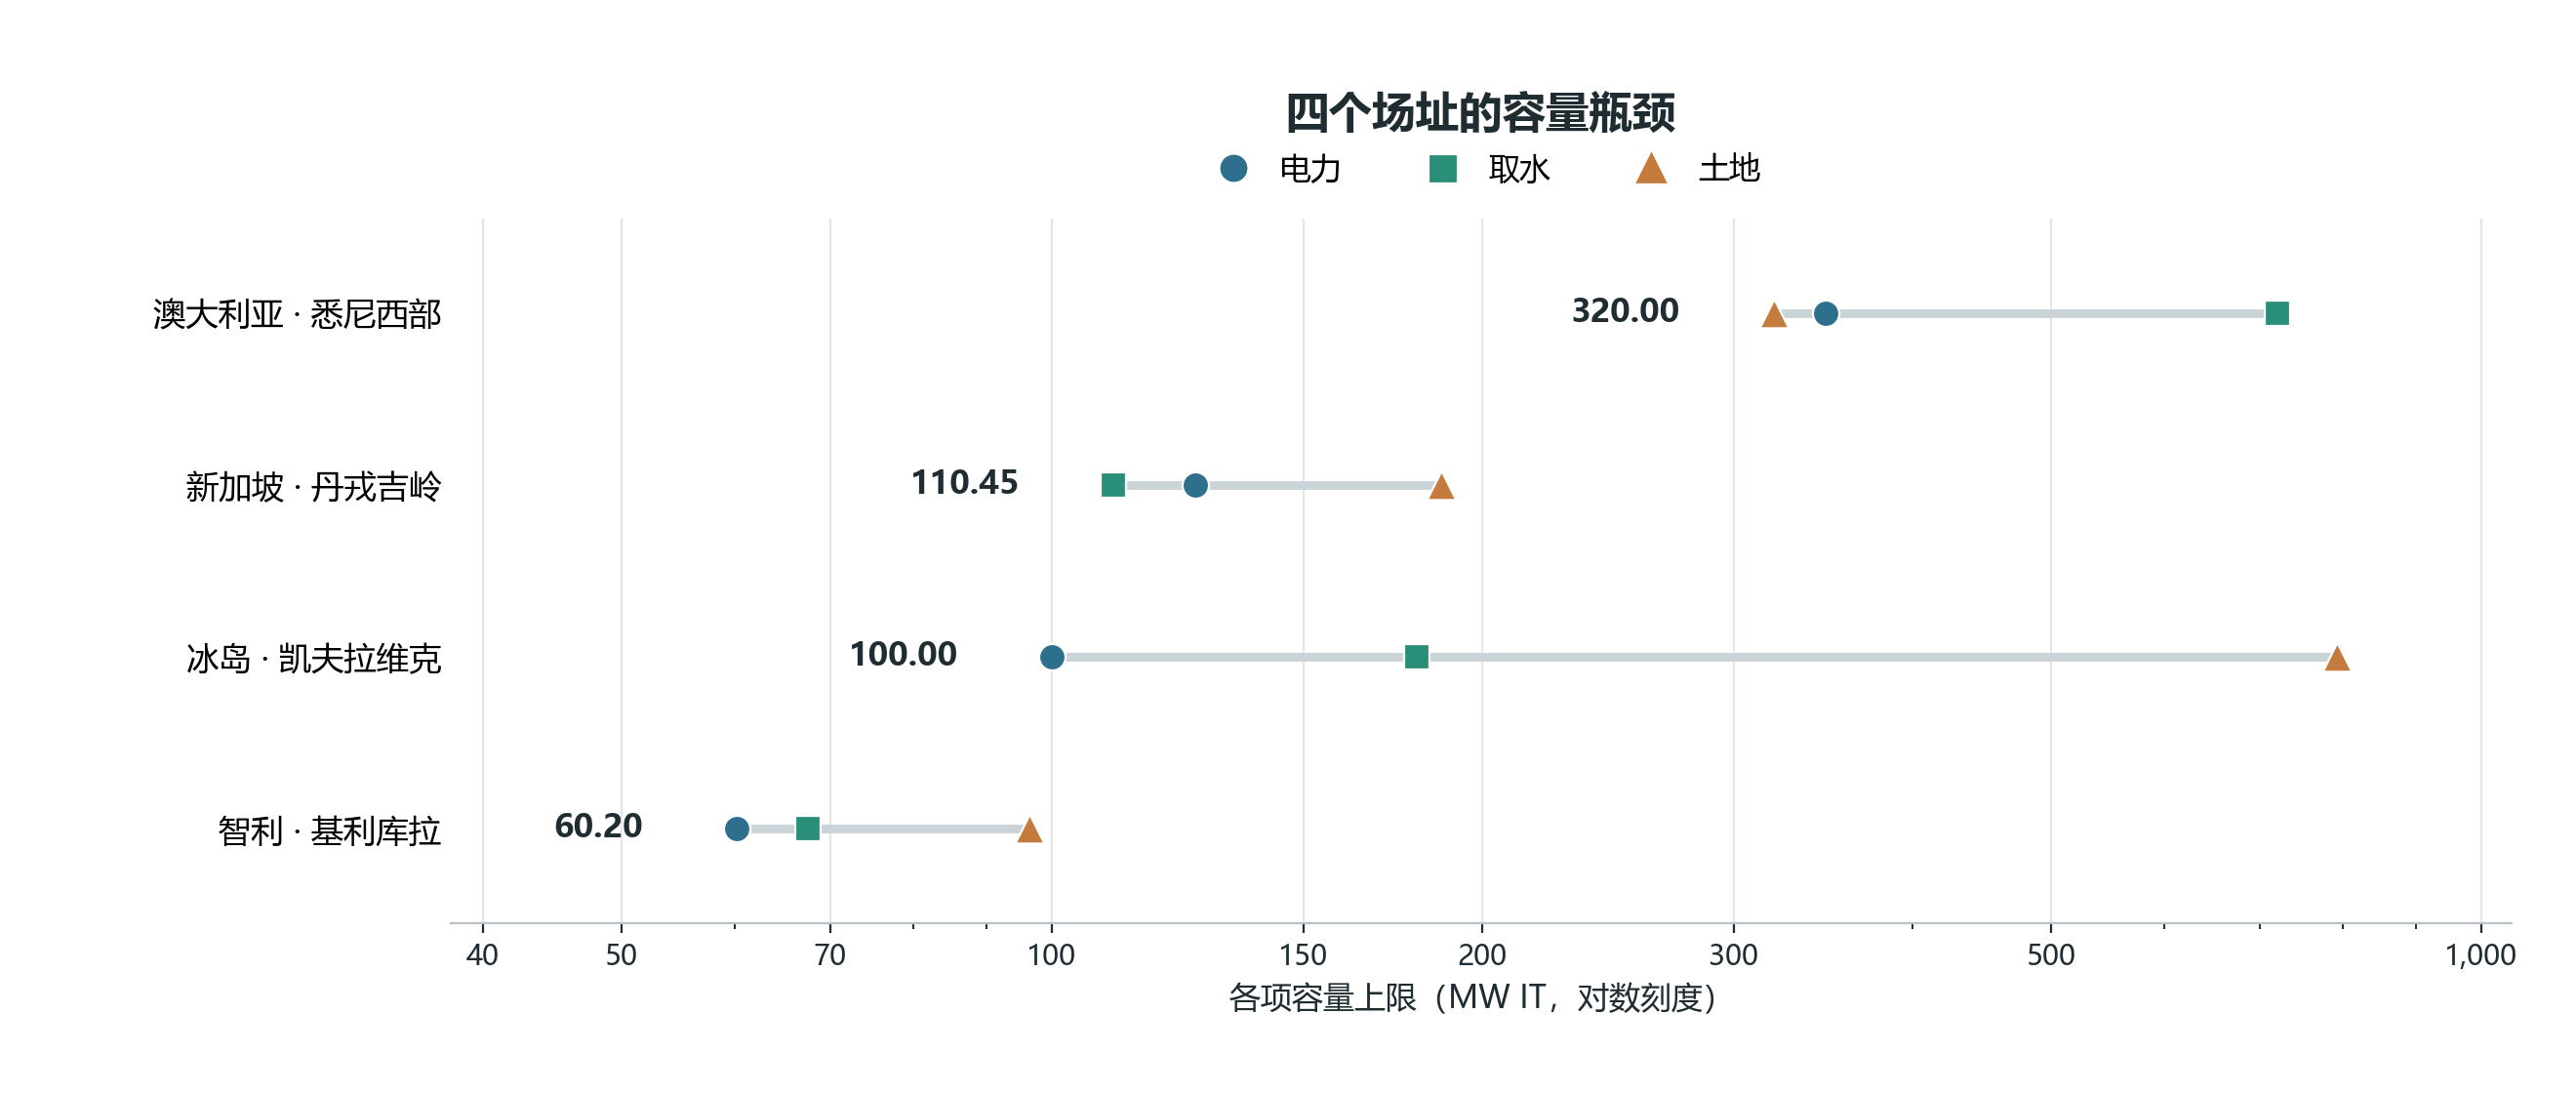
\includegraphics[width=0.76\textwidth]{figures/fig4-4.png}
\caption{四个对比场址的三项资源上限与瓶颈归属。圆点、方块、三角分别为电力、取水与土地单项上限；每行最左侧的标记与标注值即该址联合取小后的基准可持续容量。}
\label{fig:four-sites}
\end{figure}

三点结论。

\begin{enumerate}[leftmargin=2em]
\item \textbf{容量与瓶颈高度场址化。} 四处基准上限分布在 $60.20$–$320.00$ MW IT：凯夫拉维克与基利库拉同主案例一样先受制于电力，丹戎吉岭受制于水（$110.45$），悉尼西部受制于土地（$320.00$）。表~\ref{tab:four-sites} 第 5 列比第 4 列更值得注意：改造实测、运营披露、市场研究代理、需求预测与审批包络被放进同一张表，不加区分地取任何一个当“真值”，都会把口径差当成模型误差。

\item \textbf{电源排序在土地紧缺处逆转。} 四处都容不下 $20$ ha 煤电模块。冰岛与智利划出同样的 $10$ ha 给燃机：凯夫拉维克土地上限 $792.50\to292.50$ 仍高于电力，联合上限由 $100.00$ 升到 $136.36$（随后转水）；基利库拉总用地仅 $15.90$ ha，扣固定 $2.03$ ha 再划 $10$ ha 只剩 $3.87$ ha，土地上限压到 $26.92$，反而比纯网电腰斩，最优扩展转为约 $5.21$ ha 地面光储（$60.23$）。判据只需一个量：土地上限与电力上限之比——凯夫拉维克约 $7.9$，基利库拉约 $1.6$；两址的小风机按厂家功率曲线折算后装机不足 $1$ MW，不改变结论。\cite{apxref28}

\item \textbf{水压力、生态与外推风险。} Aqueduct 基线压力比显示基利库拉（$4.25$）处于极高压力流域，悉尼西部（$0.50$）高，凯夫拉维克（$0.017$）与丹戎吉岭（$0.043$）低；这与第~\ref{sec:q1-water}~节的 $S\le S_{\max}$ 判据是同一类指标——$S$ 问流域还剩多少余量，$P_W$ 问项目能拿到多少可送达流量。基利库拉的井群若从水权 $50$ L/s 回落到设计平均 $15$ L/s，上限由 $60.20$ 跌到 $20.28$。生态敏感性以“只用已批复园区”处理：四处均为已建或已核准项目，约束以许可边界与可用连续地块上界进入；若折算为有效用地折减 $10\%$／$20\%$，阿比林仍有 $979$／$870$ MW IT（结论不变），而土地先触顶的悉尼西部会从 $320.00$ 掉到 $288.0$／$256.0$。三者说明外推到新场址必须先取得旱季保障配水量、可交付网电份额与真实可用占地，缺一项就会高估水与电网的支撑力。
\end{enumerate}

综合四组证据：同址同阶段模型偏高 $3.28\%$，差额可拆到口径与阶段；换场址后容量与瓶颈逐址可解释。差异中来自资源禀赋的部分无法通过配置消除，来自口径与阶段的部分则可以通过统一口径对齐



